\documentclass[a4paper]{article}
\usepackage[UTF8]{ctex}
\usepackage{geometry}
\usepackage{graphicx}
\usepackage{url}
\usepackage{multirow}
\usepackage{array}
\usepackage{booktabs}
\usepackage{url}
\usepackage{enumitem}
\usepackage{graphicx}
\usepackage{float}
\usepackage{amssymb}
\usepackage{amsmath}
\usepackage{subfig}
\usepackage{longtable}
\usepackage{pifont}
\usepackage{color}

\allowdisplaybreaks

\geometry{a4paper, scale=0.78}

\usepackage{tikz}
\newcommand*{\circled}[1]{\lower.7ex\hbox{\tikz\draw (0pt, 0pt)%
    circle (.5em) node {\makebox[1em][c]{\small #1}};}}
    

% \begin{figure}[H]
%     \centering
%     \includegraphics[width=.55\textwidth]{E.png}
%     \caption{矩阵与列向量的乘法}
%     \label{fig:my_label_1}
% \end{figure}

% \left\{
% \begin{array}{ll}
%       x+2x+z=2 & \\
%       3x+8y+z=12 & \\
%       4y+z=2
% \end{array}
% \right.

% \begin{enumerate}[itemindent = 1em, itemsep = 0.4pt, parsep=0.5pt, topsep = 0.5pt]

% \end{enumerate}

%\stackrel{a}{\longrightarrow}

%\underbrace{}_{} %下括号

%\tableofcontents %目录,并且目录页不记录页码
% \tableofcontents
% \newpage
% \setcounter{page}{1} %new page
% \clearpage

\title{Flow Model}
\author{Chen Gong}
\date{27 June 2020}
\begin{document}
\maketitle

\section{Introduction}
在上一小节中讲到了Latent Variable Model(LAM),VAE。其主要思想就是将隐变量扩充为高维连续的分布,来增强模型的表达能力。而LAM模型中的核心困难是$P(X)$计算不出来,因为$P(X) = \int_Z P(X|Z)P(Z) dZ$,而$Z$的维度过高$P(X)$算不出来。而根据Bayesian公式:
\begin{equation}
    P(Z|X) = \frac{P(Z)P(X|Z)}{P(X)}
\end{equation}
所以导致$P(Z|X)$无法计算。而VAE那章介绍了近似推断的方法,使用一个简单分布$Q_\phi(Z|X)$来近似$P(Z|X)$,其中还使用重参数化技巧来用一个神经网络来代替分布。

而在VAE中通过优化变分下界ELBO来达到最终优化的目的,而不是直接对Log似然函数进行优化。所以当然会有误差了。那么这将启发我们,可不可以绕过这个intractable的$P(Z)$,使模型变得tractable。

\section{Flow based Model}
什么是flow model呢?首先用一张图来进行表示:
\begin{figure}[H]
    \centering
    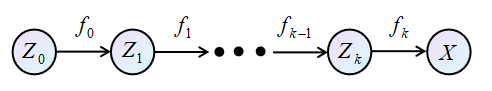
\includegraphics[width=.55\textwidth]{微信图片_20200628202302.png}
    \caption{Flow模型基础示意图}
    \label{fig:my_label_1}
\end{figure}
可以用一个简单的例子来简单的介绍Flow model。$X$可以代表是当前的自己,人是比较复杂的,所以$X \to P_X(X)$计算非常困难。而一般昨天的我$Z_k \to P_{Z_k}(Z_k)$,比今天要简单一点,但是很有可能,昨天的我依然很复杂,无法计算。那么,就不但的往前推,到了刚出生的时候$Z_0$,这时肯定是非常简单的,$Z_0 \to P_{Z_0}(Z_0)$婴儿的世界里是非黑即白的,此时的分布很简单,可以被假设为$\mathcal{N}(0,I)$。而这个过程:
\begin{equation}
    P_{Z_0}(Z_0) \to P_{Z_1}(Z_1) \to P_{Z_2}(Z_2) \cdots \to P_{Z_k}(Z_k) \to P_{X}(X)
\end{equation}
就被称为“流”。因为流模型中初始分布是很简单的。极大似然估计中求的是:$\arg\max P(X)$。那么下一个问题就是如何建立$X$和$Z_0$之间的关系,将$\arg\max P(X)$转换成求关于$P(Z_0)$的函数。

\section{Change of Variables}
假设$X=f(Z)$,$Z,X\in \mathbb{R}^p$。而$Z\sim P_Z(Z)$,$X\sim P_X(X)$;$f$是一个光滑可逆的函数。

那么可以得到:
\begin{equation}
    \int_Z P_Z(Z) dZ = 1 = \int_X P_X(X) dX
\end{equation}
根据不定积分的性质可以得到:
\begin{gather}
    |P_Z(Z) dZ| = |P_X(X) dX| \\
    P_X(X) = \left| \frac{dZ}{dX} P_Z(Z) \right|
\end{gather}
而$X=f(Z)$且$f$是光滑可逆的,所以$Z = f^{-1}(X)$,那么有
\begin{equation}
    P_X(X) = \left| \frac{\partial f^{-1}(X)}{\partial X}  \right|P_Z(Z)
\end{equation}
但是实际上$Z$和$X$都是高维变量,所以$\frac{\partial f^{-1}(X)}{\partial X}$是一个Jacobian Matrix。\textbf{熟悉矩阵的朋友应该知道,矩阵代表了一个变换,而矩阵行列式的值则代表了变换的尺度。}而在计算中我们关注的是矩阵变换的尺度,所以,
\begin{equation}
    P_X(X) = \left| \text{det}\left( \frac{\partial f^{-1}(X)}{\partial X} \right)  \right|P_Z(Z)
\end{equation}
而最终的目的是想将$P_X(X)$完全用一个$Z$为自变量的函数来表达,所以要将$\left| \frac{\partial f^{-1}(X)}{\partial X} \right|$用$Z$来表示。下面先写结论
\begin{equation}
    \begin{split}
         P_X(X) = & \left| \text{det}\left( \frac{\partial f^{-1}(X)}{\partial X} \right)  \right|P_Z(Z) \\
         = & \left| \text{det}\left( \frac{\partial f^{-1}(Z)}{\partial Z} \right)  \right|^{-1}P_Z(Z)
    \end{split}
\end{equation}

这个结论是怎么来的呢?我们来看一个简单的例子,如下图所示:
\begin{figure}[H]
    \centering
    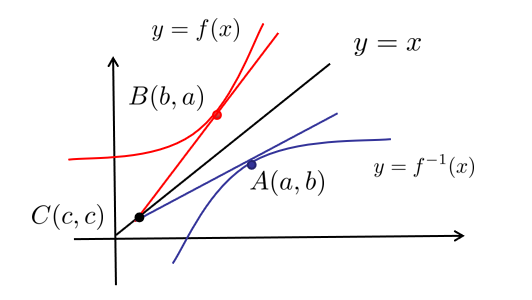
\includegraphics[width=.55\textwidth]{微信图片_20200629094542.png}
    \caption{实例}
    \label{fig:my_label_1}
\end{figure}
如图所示,$y=f(x)$,$x=f^{-1}(y)$。那么有
\begin{equation}
    \frac{dy}{dx} = \frac{\partial f(x)}{\partial x}, \frac{dx}{dy} = \frac{\partial f^{-1}(y)}{\partial y}
\end{equation}
而,
\begin{equation}
    \frac{\partial f(x)}{\partial x} \frac{\partial f^{-1}(y)}{\partial y} = 1
\end{equation}
在本文举的例子中,
\begin{equation}
\begin{split}
    (f^{-1})'(a) = \frac{b-c}{a-c} \\
    (f)'(b) = \frac{a-c}{b-c} 
\end{split}
\end{equation}
很显然有$(f^{-1})'(a) f'(b) = 1$。这就是change of
variables theorem。我们可以得到两个变量之间关于映射$f$的转换为:
\begin{equation}
    \begin{split}
         P_X(X) = & \left| \text{det}\left( \frac{\partial f^{-1}(Z)}{\partial Z} \right)  \right|^{-1}P_Z(Z)
    \end{split}
\end{equation}
\textbf{那么,当训练完成之后,从$P(Z)$中采样比较简单,通过上述公式,就可以得到$P(X)$,所以$P(X)$是可求解的。}如何学习呢?其实并不难,通过极大似然估计可以得到:
\begin{equation}
    \log P_X(X) = \log \left| \text{det}\left( \frac{\partial f^{-1}(Z)}{\partial Z} \right)  \right|^{-1} + \log P_Z(Z)
\end{equation}
那么:
\begin{equation}
\begin{split}
    \frac{\partial \log P_X(X)}{\partial X} = & \frac{\partial \log \left| \text{det}\left( \frac{\partial f^{-1}(Z)}{\partial Z} \right)  \right|^{-1} + \log P_Z(Z)}{ \partial Z} \frac{\partial Z}{ \partial X} \\
    = & \frac{\partial \log \left| \text{det}\left( \frac{\partial f^{-1}(Z)}{\partial Z} \right)  \right|^{-1} + \log P_Z(Z)}{ \partial Z} \frac{\partial f^{-1}(X)}{ \partial X}
\end{split}
\end{equation}
由于$f$的逆很要求,上述梯度的计算还是比较简单的。然而,关于大矩阵行列式的计算并不美丽。后续有很多针对这点的改进方法,有兴趣的同学自行查看flow based的论文。

[1] ICLR 2015 NICE-Non-linear Independent Components Estimation

[2] ICLR 2017 Density estimation using Real NVP

[3] 2018 Glow: Generative Flow with Invertible 1×1 Convolutions

\section{小结}
本章主要介绍的是流模型的主要思想,在Latent Variable Model经常会遇到后验过于复杂无法求解的问题。流模型绕开了这个部分,对更简单的分布建模,然后建立原分布与简单分布之间的映射关系。个人觉得Stein变分梯度下降就有点流模型的影子在里面。在建立映射关系是用到了重要的change of variables theorem,并之后介绍了变化后的目标函数和梯度求解方法。


\end{document}
